% Declare type of document
\documentclass[10pt]{article}

% Import Packages
\usepackage[utf8]{inputenc} 

% Commonly used math symbols and fonts
\usepackage[mathscr]{euscript}
\usepackage{amsfonts,amsmath,amssymb,amsthm}
\usepackage{mathtools,mathdots}

% Better looking default font
\usepackage{lmodern}

% itemize environment
\usepackage{enumitem}
\usepackage{enumerate}

% Array, longtable, and booktabs
\usepackage{array}
\usepackage{longtable}
\usepackage{booktabs}
 
% Caption package for hiding Figure #
\usepackage{caption}

% Page formatting
\usepackage[letterpaper, margin=1in]{geometry}

% Package for nice syntax highlighting for code
% \usepackage[cache=false]{minted}
\usepackage{minted} 

% Allows line breaks in the math environment
\allowdisplaybreaks

\usepackage[activate={true,nocompatibility},final,tracking=true,kerning=true,spacing=true,factor=1100,stretch=10,shrink=10]{microtype}
\microtypecontext{spacing=nonfrench}
% activate={true,nocompatibility} - activate protrusion and expansion
% final - enable microtype; use "draft" to disable
% tracking=true, kerning=true, spacing=true - activate these techniques
% factor=1100 - add 10% to the protrusion amount (default is 1000)
% stretch=10, shrink=10 - reduce stretchability/shrinkability (default is 20/20)


\title{CS 310: Trees (Part II)}
\author{Connor Baker}
\date{February 21, 2019}

\begin{document}

\maketitle

\subsection*{Recursion Example}
\begin{itemize}
    \item Binary tree \mintinline{java}{.size()} counts the number of nodes in a tree
    \item Recursive helper: \mintinline{java}{.size(Node n)} that counts the number of nodes in a sub-tree rooted at the node including itself
    \begin{itemize}
        \item Base case: the size of \mintinline{java}{null} is zero
        \item Recursive case: Size of tree = \mintinline{java}{size(node.left)} + \mintinline{java}{size(node.right)} + 1
    \end{itemize}
    \item We could implement this as
    \begin{minted}{java}
// Recursive method to count
public static <T> int size(Node<T> t) {
    if (t == null) {
        return 0;
    }
    int sL = size(t.left);
    int sR = size(t.right);
    return 1 + sL + sR;
}
    \end{minted}
    \item Exercise: define a recursive function \mintinline{java}{.height(Node n)} that returns the height of a tree node
    \begin{itemize}
        \item Length of the longest path from a node to a leaf
        \item Leaf node height is zero
    \end{itemize}
    
\end{itemize}

\subsection*{Common Tree Operations}
\begin{itemize}
    \item Searching for an item
    \item Adding items
    \item Deleting items
    \item Balancing
    \item Iteration (either through all of the tree, or a sub-tree)
\end{itemize}

\subsection*{Tree Traversals}
\begin{itemize}
    \item Check Weiss 18.4: traversal implementation in an iterator
    \item Two common types:
    \begin{center}
        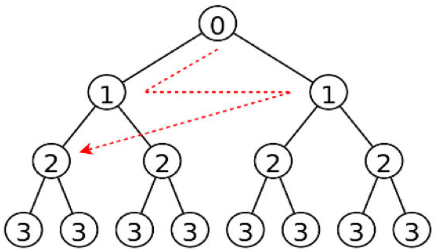
\includegraphics[width=0.35\textwidth]{images/1.png}
        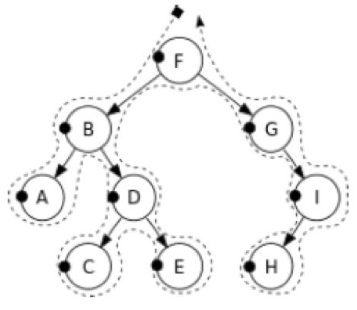
\includegraphics[width=0.25\textwidth]{images/2.png}
    \end{center}
    \begin{itemize}
        \item (Left) \textit{Breadth first search}: a search which proceeds by processing all nodes level by level, with those closest to the root processed first
        \item (Right) \textit{Depth first search}: a search which proceeds by following a path all the way to a leaf and then backtracking
    \end{itemize}
\end{itemize}

\subsection*{Depth First Traversal}
\begin{itemize}
    \item The walking of a tree starts with the root and goes from parent to child
    \item There are three different orders we can ``process'' the nodes in:
    \begin{enumerate}[(a)]
        \item Pre-order traversal (parent, left, right)
        \item Post-order traversal (left, right, parent)
        \item In-order traversal (left, parent, right)
    \end{enumerate}
\end{itemize}
\begin{center}
    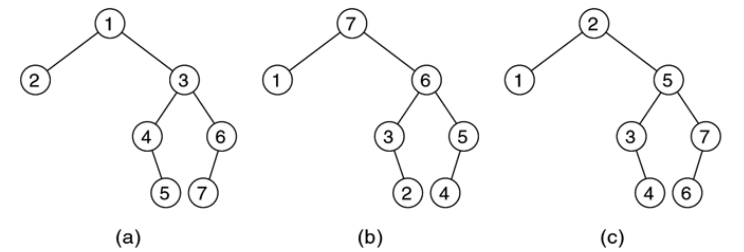
\includegraphics[width=0.75\textwidth]{images/3.png}
\end{center}

\subsection*{Traversal Examples}
\begin{center}
    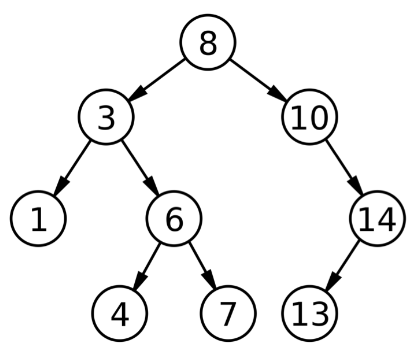
\includegraphics[width=0.25\textwidth]{images/4.png}
\end{center}
\begin{itemize}
    \item For the given tree, show
    \begin{itemize}
        \item Pre-order traversal
        \begin{itemize}
            \item $8,3,1,6,4,7,10,14,13$
        \end{itemize}
        \item Post-order traversal
        \begin{itemize}
            \item $1,4,7,6,3,13,14,10$
        \end{itemize}
        \item In-order traversal
        \begin{itemize}
            \item $1,3,6,7,4,10,13,14$
        \end{itemize}
    \end{itemize}
    \item Which one sorts the nodes according to their data?
    \begin{itemize}
        \item That would be a special feature of binary search trees under an in-order traversal
    \end{itemize}
\end{itemize}

\section*{Implementing Traversal for Binary Trees}
\begin{minipage}[t]{0.5\linewidth}
\begin{minted}[linenos=true]{java}
class Node<T> {
    T data;
    Node<T> left, right;
}

inOrder(Node t) {
    if (t == null) {
        return;
    }

    inOrder(t.left);
    print(t.data);
    inOrder(t.right);
}

// to use
inOrder(this.root);
\end{minted}    
\end{minipage}%
\begin{minipage}[t]{0.5\linewidth}
\begin{minted}[linenos=true,firstnumber=18]{java}
preOrder(Node t) {
    if (t == null) {
        return;
    }

    print(t.data);
    preOrder(t.left);
    preOrder(t.right);
}

postOrder(Node t) {
    if (t == null) {
        return;
    }

    postOrder(t.left);
    postOrder(t.right);
    print(t.data);
}
\end{minted}    
\end{minipage}

\subsection*{Notes on the Tree Traversal Implementation}
\begin{itemize}
    \item The recursive approach is easy to code
    \item The time and space complexity isn't great, however
    \item We can perform various operations on each node following different orders
\end{itemize}

\subsection*{Traversal Example}
\begin{itemize}
    \item Binary tree \mintinline{java}{.size()} method, which counts how many nodes a tree contains
\begin{minted}{java}
// Recursive method to count the number of nodes
public static <T> int size(Node<T> t) {
    if (t == null) {
        return 0;
    }

    int sL = size(t.left);
    int sR = size(t.right);

    return 1 + sL + sR;
}
\end{minted}
    \item In what order are we processing the nodes? Why?
    \begin{itemize}
        \item Post-order: if we have a sorted binary tree, it gives us the elements in order
    \end{itemize}
\end{itemize}

\subsection*{Tree Traversal Examples}
\begin{itemize}
    \item Task: mark the depth of every node
    \begin{itemize}
        \item What order should we use?
        \item \textbf{Practice}: write the recursive code
    \end{itemize}
    \item Task: check whether the (binary) tree is balanced
    \begin{itemize}
        \item Order?
        \item \textbf{Practice}: write the recursive code
    \end{itemize}
\end{itemize}

\subsection*{Iterative Tree Traversal}
\begin{itemize}
    \item Can we implement tree traversal without recursion?
    \begin{itemize}
        \item Well... yes, but we need to maintain a stack (which is what recursion does for us)
    \end{itemize}
    \item We can check the post-order traversal. Every node needs to go through three steps in order:
    \begin{itemize}
        \item Process the node's left subtree
        \item Process the node's right subtree
        \item Process the node itself
    \end{itemize}
\end{itemize}

\subsection*{Iterative Implementation of Traversal}
\begin{minted}{java}
// Pseudo-code for post-order printing
void postOrder(root) {
    Stack s = new Stack();
    s.push({root, DOLEFT});
    while (!s.isEmpty()) {
        {tree, action} = s.popTop();
        if (tree == null) {
            // Do nothing
        } else if (action == DOLEFT) {
            s.push({tree, DORIGHT});
            s.push({tree.left, DOLEFT});
        } else if (action == DORIGHT) {
            s.push({tree, DOTHIS});
            s.push({tree.right, DOLEFT});
        } else if (action == DOTHIS) {
            print(tree.data);
        } else {
            throw new YouScrewedUpException();
        }
    }
}
\end{minted}
\begin{itemize}
    \item Use an explicit stack
    \begin{itemize}
        \item Push the node onto the stack three times, each with a different task
    \end{itemize}
    \item Auxiliary data action
    \item \mintinline{java}{DOLEFT} works on the left sub-tree
    \item \mintinline{java}{DORIGHT} works on the right sub-tree
    \item \mintinline{java}{DOTHIS} processes data for the current node
\end{itemize}

\subsection*{Iterative Post-Order Traversal}
\begin{center}
    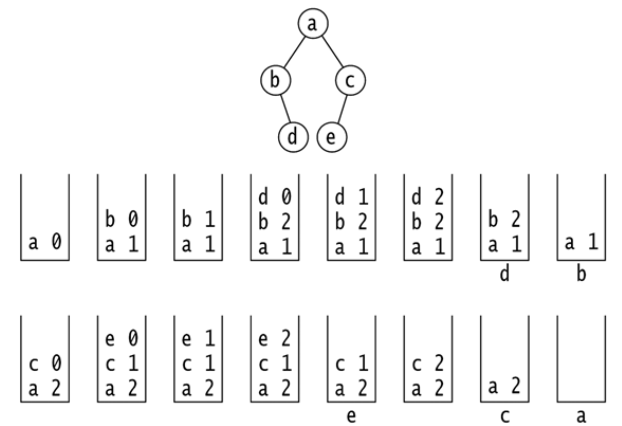
\includegraphics[width=0.5\linewidth]{images/5.png}
\end{center}
\begin{itemize}
    \item Stack status:
    \begin{itemize}
        \item 0: \mintinline{java}{DOLEFT}
        \item 1: \mintinline{java}{DORIGHT}
        \item 2: \mintinline{java}{DOSELF}
    \end{itemize}
\end{itemize}

\subsection*{Iterative Tree Traversal}
\begin{itemize}
    \item Recursive implementations are easier to code but generally cost more memory
    \item Iterative methods are possible and save memory at the expense of tricky code
    \begin{itemize}
        \item Pre-order and in-order follow the same idea as post-order
        \item We can augment tree noes to have a reference to their parent
        \begin{itemize}
            \item \mintinline{java}{class Node<T> {T data; Node left, right, parent;}}
        \end{itemize}
        \item This enables stack-less, iterative traversals with great cleverness
    \end{itemize}
\end{itemize}

\subsection*{Weiss' Traversals}
\begin{minted}{java}
BinaryTree<Integer> t = new BinaryTree<>();
// fill the tree
TreeIterator<T> itr = new PreOrder<Integer>(t);
for (itr.first(); itr.isValid(); itr.advance()) {
    System.out.println(" " + itr.retrieve());
}
\end{minted}
\begin{itemize}
    \item Weiss' traversals are implemented as iterators
    \begin{itemize}
        \item More complex to understand, but generally easier to use
        \item Play with some of these if you want more practice
    \end{itemize}
\end{itemize}

\subsection*{Breadth First Traversal}
\begin{center}
    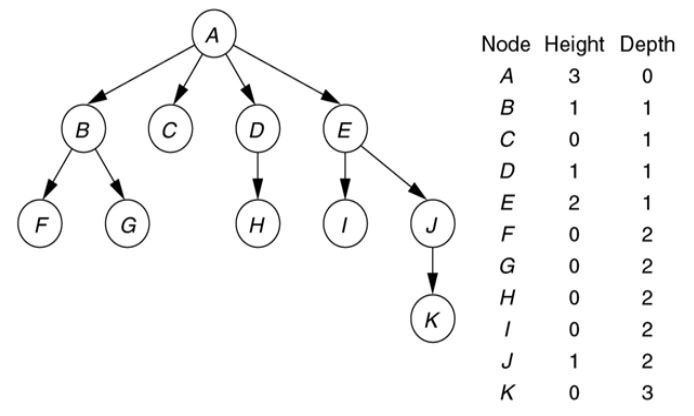
\includegraphics[width=0.5\linewidth]{images/6.png}
\end{center}
\begin{itemize}
    \item Level-order traversal: visit the nodes from top to bottom, left to right
    \begin{itemize}
        \item $A \to B \to C \to D \to E \to F \to G \to H \to I \to J \to K$
    \end{itemize}
    \item If you're using an array, you can walk the array
    \item If you're using a linked list, you can use a queue
\end{itemize}

\subsection*{Next Lecture}
\begin{itemize}
    \item Summary: tree basis
    \begin{itemize}
        \item Definitions
        \item Operations
        \item Recursion review
    \end{itemize}
    \item Next lecture: Hashing
    \begin{itemize}
        \item Reading: Chapter 20
    \end{itemize}
\end{itemize}

\end{document}